\subsubsection{Proton}

Figure\ref{fig:Proton_Event_Display} shows typical event of proton.
Proton has simple structure of events because proton doesn't decay any particles.
Therefore, it is easy to define stopped point.
First, protons are selected by the information of beam counters.
Then, proton events are applied following simple selections.\\

\begin{enumerate}
\item The time of the hit of the minimum channel number in the cluster is between 354.8ns$\sim$504.8ns(this time window is signal region). \\
\item The minimum channel number of hits in the cluster is below 2. \\
\item The maximum channel number of hits in the cluster is below 60. \\
\item The total hit number in the cluster is 5 or more. \\
\item The number of hits which are in the same channel is only one. \\
\end{enumerate}

We define the events which the number of clusters in the event which passed above selections is only one as good proton events.
For protons was chosen in a such way, we define the hit which has the maximum channel number as stopped point.
It should noted that stopped point include fake hit in a proportion because of the influence of cross talk as described in section 6.6.\\

\begin{figure}[htbp]
  \centering
  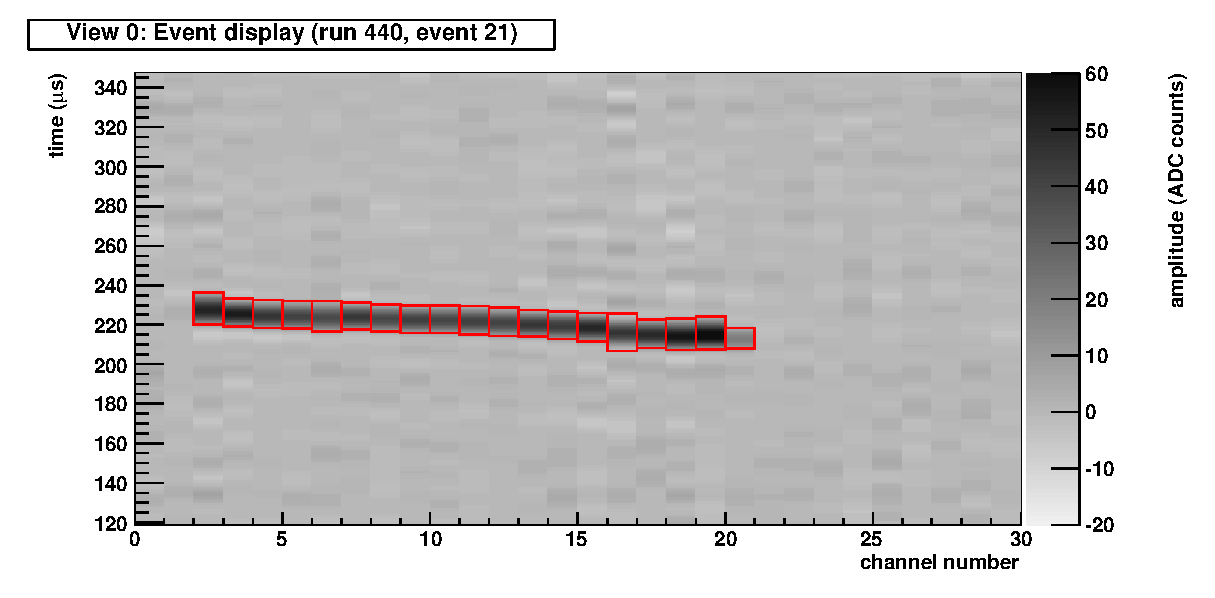
\includegraphics[width=10cm,clip]{./fig/Display_run440_ev21.eps}
  \caption{Typical Event Display of Proton}
  \label{fig:Proton_Event_Display}
\end{figure}
